\documentclass[a4paper]{article}

\usepackage{showcode/showcode}
\usepackage{amssymb}
\usepackage{amsthm}
\usepackage{mathtools}
\usepackage{bm}

% \begin{center}
% \showc*[.75\textwidth]{test.c}
% \end{center}

% \begin{Listing} % [ht]
%     \centering
%         \showc*[.5\textwidth]{test.c}
%         \caption{A C program.}\label{c}
% \end{Listing}

\usepackage[a4paper]{geometry}
\usepackage[hidelinks]{hyperref}
\usepackage{eurosym}
\usepackage{caption, subcaption}
\usepackage{tikz, circuitikz}
\usepackage{pgf-umlcd, pgf-umlsd}
\usepackage[italian]{babel}
\usepackage[utf8]{inputenc}
\usepackage[T1]{fontenc}
\usepackage[normalem]{ulem}

\renewcommand{\umltextcolor}{black}
\renewcommand{\umldrawcolor}{black}
\renewcommand{\umlfillcolor}{white}

\definecolor{type}{RGB}{132, 42, 17}

% \setlength{\parskip}{1.2ex}
% \setlength{\parindent}{0em}
% \clubpenalty = 100
% \widowpenalty = 100

% \title{CHIP-8 STM32}
% \date{\today}
% \author{Federico Bruzzone, Lorenzo Ferrante, Andrea Longoni \\
% \footnotesize \texttt{\{federico.bruzzone, lorenzo.ferrante1, andrea.longoni3\}@studenti.unimi.it} \\ }



\textwidth=450pt
\oddsidemargin=0pt
\textheight=665pt
\voffset=-50pt

% \singlespacing

\begin{document}
% \maketitle
% \newpage

\begin{titlepage}
	\begin{center}
		
\includegraphics[height=5cm]{minerva.pdf}

		\vspace*{1.75cm}

		\LARGE

		\textbf{MSc in Computer Science} \\
		at University of Milan

		\vspace*{1cm}

		\huge
		CHIP-8 STM32

		\large Proposta per il Progetto di PROS, \\
		corso tenuto da \textbf{Danilo Bruschi}

		\normalsize
		\vspace*{4cm}

		\begin{minipage}[t]{0.47\textwidth}
			{Email: } \vspace{0.3em} \\
			{\large \href{federico.bruzzone@studenti.unimi.it}{federico.bruzzone@studenti.unimi.it}} \vspace{1em}  \\
			{\large \href{lorenzo.ferrante1@studenti.unimi.it}{lorenzo.ferrante1@studenti.unimi.it}} \vspace{1em}  \\
			{\large \href{andrea.longoni3@studenti.unimi.it}{andrea.longoni3@studenti.unimi.it}} \vspace{1em}  \\
		\end{minipage}
		\hfill
		\begin{minipage}[t]{0.47\textwidth}\raggedleft
			{Creato da:} \hspace{-0.9em} \vspace{0.3em} \\
			{\large \textbf{Federico Bruzzone}} \\
			\vspace{1em}
			{\large \textbf{Lorenzo Ferrante}} \\
			\vspace{1em}
			{\large \textbf{Andrea Longoni}}
		\end{minipage}

		\vfill
		Anno accademico 2022/2023

	\end{center}
\end{titlepage}
\setlength{\parindent}{0pt}
\setlength{\parskip}{0.8em}
% \linespread{1.5}

\tableofcontents
\listoffigures
\listoftables

\newpage

\section{Introduzione}

% TODO: includere una foto dell'emulatore finito e funzionante

CHIP-8 è un linguaggio di programmazione creato a metà degli anni '70
da Joseph Weisbecker per semplificare lo sviluppo di videogiochi per
microcomputer a 8 bit. I programmi CHIP-8 vengono interpretati da una
macchina virtuale che è stata estesa parecchie volte nel corso degli
anni, tra le versioni più adottate citiamo S-CHIP e la più recente
XO-CHIP.

La semplicità dell'interprete in aggiunta alla sua lunga storia e
popolarità hanno fatto sì che emulatori e programmi CHIP-8 vengano
realizzati ancora oggi.
Nel corso degli anni molti videogiochi storici sono stati riscritti
in CHIP-8 tra cui Pong, Space Invaders e Tetris.

Lo scopo del progetto è quello di costruire un emulatore CHIP-8 e
S-CHIP in grado di funzionare su un microcontrollore STM32.

In questo documento ci riferiremo alla macchina virtuale che
interpreta programmi CHIP-8 con "interprete". Mentre utilizzeremo
"emulatore" per indicare l'interprete assieme ad una sua
implementazione (o "port"), ovvero un programma che gestisce
l'audio, il video, l'input da tastiera e interagisce con l'API della
macchina virtuale.

\section{Stato dell'arte}

Al giorno d'oggi risulta difficile ottenere un numero esatto di utenti che utilizzano CHIP-8, un buon indicatore puo' essere il topic "chip8" di GitHub che raggruppa quasi un migliaio di repository.

Tra queste la più popolare è Octo, un'implementazione scritta in JavaScript capace di eseguire la versione base di CHIP-8, S-CHIP e XO-CHIP nel browser. La repository è mantenuta da John Earnest, l'inventore di XO-CHIP che nel 2014 ha riportato in vita CHIP-8 modernizzandolo e aggiungendo nuove funzionalità.

Inoltre ogni anno viene organizzata la Octojam, una game jam dove ogni partecipante prova a sviluppare un videogioco per CHIP-8 (o per le sue estensioni) partendo da zero.

Grazie al suo instruction set ridotto e alla sua limitata richiesta di risorse hardware è stato portato su un elevato numero di piattaforme, tra cui il Game Boy Color, calcolatrici grafiche serie HP 48 e Emacs (il famoso editor di testo).

Sebbene CHIP-8 e S-CHIP siano stati tradizionalmente implementati tramite software esistono anche implementazioni hardware. Ne citiamo una in particolare scritta nel linguaggio Verilog per schede FPGA.

\section{Hardware}\label{sec:hardware}

Le componenti principali utilizzate per la relizzazione del progetto sono 5:
una scheda ST \texttt{STM32F334R8T6} (Fig. \ref{fig:stm32f334}), uno schermo
TFT LCD ILI9341 (Fig. \ref{fig:ili9341}), e un lettore di schede microSD
integrato nello schermo, un tastierino matriciale 4$\times$4 e un beeper.

Il componente principale é il microcontrollore \texttt{STM32F334R8T6} basato su
architettura ARM con processore Cortex-M4 da 72 \texttt{MHz}, 64 \texttt{Kb} di
memoria flash e 16 \texttt{Kb} di SRAM. Abbiamo deciso di utilizzare questa
scheda perché le ROM dei giochi CHIP-8 e S-CHIP hanno dimensione massima di 4
\texttt{Kb}. Considerando questo e il fatto che la macchina virtuale necessita
4 \texttt{Kb} per poter funzionare non è stato potuto utilizzare la scheda
\texttt{STM32L053R8T6} fornitaci durante il corso a causa della sua quantità
limita di SRAM, precisamente 8 \texttt{Kb}.

\begin{figure}[h!t]
    \begin{subfigure}[b]{0.45\textwidth}
        \begin{center}
            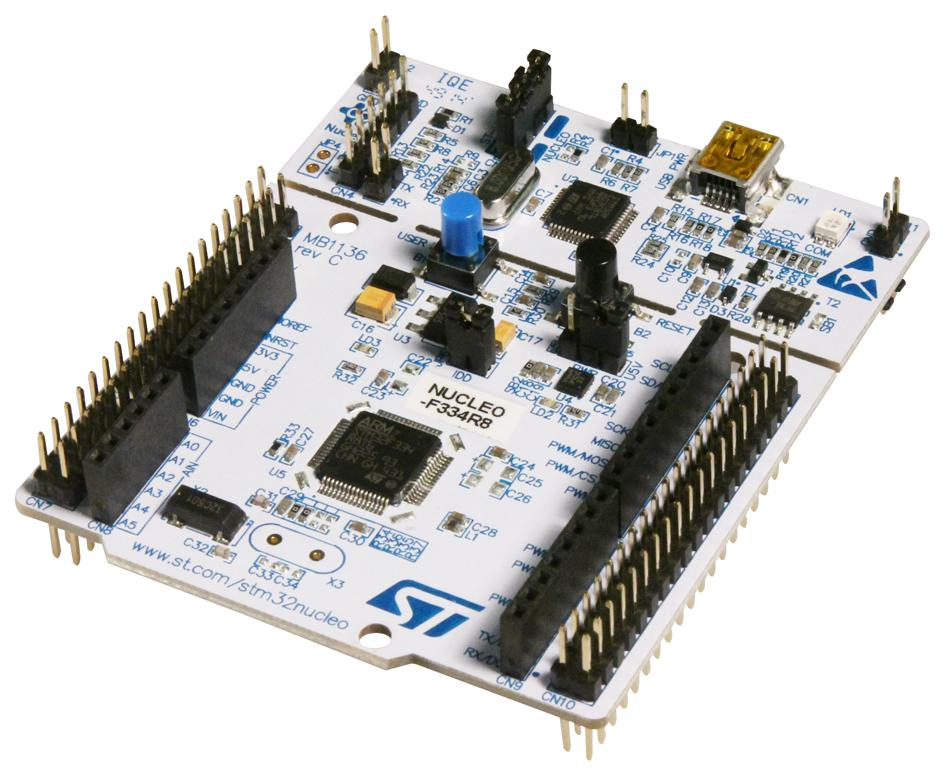
\includegraphics[scale=0.15]{figures/stm32f334.jpg}
        \end{center}
        \caption{Il microcontrollore \texttt{STM32F334R8T6}.}
        \label{fig:stm32f334}
    \end{subfigure}
    \hfill
    \begin{subfigure}[b]{0.45\textwidth}
        \begin{center}
            \begin{tikzpicture}[x=0.015cm, y=0.015cm, scale=0.50, transform shape]
                % \draw  [color={rgb, 255:red, 0; green, 0; blue, 0 }  ,draw opacity=1 ][fill={rgb, 255:red, 255; green, 255; blue, 255 }  ,fill opacity=1 ] (400,140) -- (720,140) -- (720,960) -- (400,960) -- cycle ;
\draw  [color={rgb, 255:red, 0; green, 0; blue, 0 }  ,draw opacity=1 ][fill={rgb, 255:red, 255; green, 255; blue, 255 }  ,fill opacity=1 ] (400,140) -- (720,140) -- (720,920) -- (400,920) -- cycle ;

\draw  [fill={rgb, 255:red, 255; green, 255; blue, 255 }  ,fill opacity=1 ] (440,150) -- (510,150) -- (510,190) -- (440,190) -- cycle ;
\draw  [fill={rgb, 255:red, 255; green, 255; blue, 255 }  ,fill opacity=1 ] (370,150) -- (440,150) -- (440,190) -- (370,190) -- cycle ;

\draw  [fill={rgb, 255:red, 255; green, 255; blue, 255 }  ,fill opacity=1 ] (440,190) -- (510,190) -- (510,230) -- (440,230) -- cycle ;
\draw  [fill={rgb, 255:red, 255; green, 255; blue, 255 }  ,fill opacity=1 ] (370,190) -- (440,190) -- (440,230) -- (370,230) -- cycle ;

\draw  [fill={rgb, 255:red, 255; green, 255; blue, 255 }  ,fill opacity=1 ] (440,230) -- (510,230) -- (510,270) -- (440,270) -- cycle ;
\draw  [fill={rgb, 255:red, 255; green, 255; blue, 255 }  ,fill opacity=1 ] (370,230) -- (440,230) -- (440,270) -- (370,270) -- cycle ;

\draw  [fill={rgb, 255:red, 255; green, 255; blue, 255 }  ,fill opacity=1 ] (440,270) -- (510,270) -- (510,310) -- (440,310) -- cycle ;
\draw  [fill={rgb, 255:red, 255; green, 255; blue, 255 }  ,fill opacity=1 ] (370,270) -- (440,270) -- (440,310) -- (370,310) -- cycle ;

\draw  [fill={rgb, 255:red, 255; green, 255; blue, 255 }  ,fill opacity=1 ] (440,310) -- (510,310) -- (510,350) -- (440,350) -- cycle ;
\draw  [fill={rgb, 255:red, 255; green, 255; blue, 255 }  ,fill opacity=1 ] (370,310) -- (440,310) -- (440,350) -- (370,350) -- cycle ;

\draw  [fill={rgb, 255:red, 255; green, 255; blue, 255 }  ,fill opacity=1 ] (440,350) -- (510,350) -- (510,390) -- (440,390) -- cycle ;
\draw  [fill={rgb, 255:red, 255; green, 255; blue, 255 }  ,fill opacity=1 ] (370,350) -- (440,350) -- (440,390) -- (370,390) -- cycle ;

\draw  [fill={rgb, 255:red, 255; green, 255; blue, 255 }  ,fill opacity=1 ] (440,390) -- (510,390) -- (510,430) -- (440,430) -- cycle ;
\draw  [fill={rgb, 255:red, 255; green, 255; blue, 255 }  ,fill opacity=1 ] (370,390) -- (440,390) -- (440,430) -- (370,430) -- cycle ;

\draw  [fill={rgb, 255:red, 255; green, 255; blue, 255 }  ,fill opacity=1 ] (440,430) -- (510,430) -- (510,470) -- (440,470) -- cycle ;
\draw  [fill={rgb, 255:red, 255; green, 255; blue, 255 }  ,fill opacity=1 ] (370,430) -- (440,430) -- (440,470) -- (370,470) -- cycle ;

\draw  [fill={rgb, 255:red, 255; green, 255; blue, 255 }  ,fill opacity=1 ] (440,470) -- (510,470) -- (510,510) -- (440,510) -- cycle ;
\draw  [fill={rgb, 255:red, 255; green, 255; blue, 255 }  ,fill opacity=1 ] (370,470) -- (440,470) -- (440,510) -- (370,510) -- cycle ;

\draw  [fill={rgb, 255:red, 255; green, 255; blue, 255 }  ,fill opacity=1 ] (440,510) -- (510,510) -- (510,550) -- (440,550) -- cycle ;
\draw  [fill={rgb, 255:red, 255; green, 255; blue, 255 }  ,fill opacity=1 ] (370,510) -- (440,510) -- (440,550) -- (370,550) -- cycle ;

\draw  [fill={rgb, 255:red, 255; green, 255; blue, 255 }  ,fill opacity=1 ] (440,550) -- (510,550) -- (510,590) -- (440,590) -- cycle ;
\draw  [fill={rgb, 255:red, 255; green, 255; blue, 255 }  ,fill opacity=1 ] (370,550) -- (440,550) -- (440,590) -- (370,590) -- cycle ;

\draw  [fill={rgb, 255:red, 255; green, 255; blue, 255 }  ,fill opacity=1 ] (440,590) -- (510,590) -- (510,630) -- (440,630) -- cycle ;
\draw  [fill={rgb, 255:red, 255; green, 255; blue, 255 }  ,fill opacity=1 ] (370,590) -- (440,590) -- (440,630) -- (370,630) -- cycle ;

\draw  [fill={rgb, 255:red, 255; green, 255; blue, 255 }  ,fill opacity=1 ] (440,630) -- (510,630) -- (510,670) -- (440,670) -- cycle ;
\draw  [fill={rgb, 255:red, 255; green, 255; blue, 255 }  ,fill opacity=1 ] (370,630) -- (440,630) -- (440,670) -- (370,670) -- cycle ;

\draw  [fill={rgb, 255:red, 255; green, 255; blue, 255 }  ,fill opacity=1 ] (440,670) -- (510,670) -- (510,710) -- (440,710) -- cycle ;
\draw  [fill={rgb, 255:red, 255; green, 255; blue, 255 }  ,fill opacity=1 ] (370,670) -- (440,670) -- (440,710) -- (370,710) -- cycle ;

\draw  [fill={rgb, 255:red, 255; green, 255; blue, 255 }  ,fill opacity=1 ] (440,710) -- (510,710) -- (510,750) -- (440,750) -- cycle ;
\draw  [fill={rgb, 255:red, 255; green, 255; blue, 255 }  ,fill opacity=1 ] (370,710) -- (440,710) -- (440,750) -- (370,750) -- cycle ;

\draw  [fill={rgb, 255:red, 255; green, 255; blue, 255 }  ,fill opacity=1 ] (440,750) -- (510,750) -- (510,790) -- (440,790) -- cycle ;
\draw  [fill={rgb, 255:red, 255; green, 255; blue, 255 }  ,fill opacity=1 ] (370,750) -- (440,750) -- (440,790) -- (370,790) -- cycle ;

\draw  [fill={rgb, 255:red, 255; green, 255; blue, 255 }  ,fill opacity=1 ] (440,790) -- (510,790) -- (510,830) -- (440,830) -- cycle ;
\draw  [fill={rgb, 255:red, 255; green, 255; blue, 255 }  ,fill opacity=1 ] (370,790) -- (440,790) -- (440,830) -- (370,830) -- cycle ;

\draw  [fill={rgb, 255:red, 255; green, 255; blue, 255 }  ,fill opacity=1 ] (440,830) -- (510,830) -- (510,870) -- (440,870) -- cycle ;
\draw  [fill={rgb, 255:red, 255; green, 255; blue, 255 }  ,fill opacity=1 ] (370,830) -- (440,830) -- (440,870) -- (370,870) -- cycle ;

\draw  [fill={rgb, 255:red, 255; green, 255; blue, 255 }  ,fill opacity=1 ] (440,870) -- (510,870) -- (510,910) -- (440,910) -- cycle ;
\draw  [fill={rgb, 255:red, 255; green, 255; blue, 255 }  ,fill opacity=1 ] (370,870) -- (440,870) -- (440,910) -- (370,910) -- cycle ;

% \draw  [fill={rgb, 255:red, 255; green, 255; blue, 255 }  ,fill opacity=1 ] (440,910) -- (510,910) -- (510,950) -- (440,950) -- cycle ;
% \draw  [fill={rgb, 255:red, 255; green, 255; blue, 255 }  ,fill opacity=1 ] (370,910) -- (440,910) -- (440,950) -- (370,950) -- cycle ;



\draw  [fill={rgb, 255:red, 255; green, 255; blue, 255 }  ,fill opacity=1 ] (610,150) -- (680,150) -- (680,190) -- (610,190) -- cycle ;
\draw  [fill={rgb, 255:red, 255; green, 255; blue, 255 }  ,fill opacity=1 ] (680,150) -- (750,150) -- (750,190) -- (680,190) -- cycle ;

\draw  [fill={rgb, 255:red, 255; green, 255; blue, 255 }  ,fill opacity=1 ] (610,190) -- (680,190) -- (680,230) -- (610,230) -- cycle ;
\draw  [fill={rgb, 255:red, 255; green, 255; blue, 255 }  ,fill opacity=1 ] (680,190) -- (750,190) -- (750,230) -- (680,230) -- cycle ;

\draw  [fill={rgb, 255:red, 255; green, 255; blue, 255 }  ,fill opacity=1 ] (610,230) -- (680,230) -- (680,270) -- (610,270) -- cycle ;
\draw  [fill={rgb, 255:red, 255; green, 255; blue, 255 }  ,fill opacity=1 ] (680,230) -- (750,230) -- (750,270) -- (680,270) -- cycle ;

\draw  [fill={rgb, 255:red, 255; green, 255; blue, 255 }  ,fill opacity=1 ] (610,270) -- (680,270) -- (680,310) -- (610,310) -- cycle ;
\draw  [fill={rgb, 255:red, 255; green, 255; blue, 255 }  ,fill opacity=1 ] (680,270) -- (750,270) -- (750,310) -- (680,310) -- cycle ;

\draw  [fill={rgb, 255:red, 255; green, 255; blue, 255 }  ,fill opacity=1 ] (610,310) -- (680,310) -- (680,350) -- (610,350) -- cycle ;
\draw  [fill={rgb, 255:red, 255; green, 255; blue, 255 }  ,fill opacity=1 ] (680,310) -- (750,310) -- (750,350) -- (680,350) -- cycle ;

\draw  [fill={rgb, 255:red, 255; green, 255; blue, 255 }  ,fill opacity=1 ] (610,350) -- (680,350) -- (680,390) -- (610,390) -- cycle ;
\draw  [fill={rgb, 255:red, 255; green, 255; blue, 255 }  ,fill opacity=1 ] (680,350) -- (750,350) -- (750,390) -- (680,390) -- cycle ;

\draw  [fill={rgb, 255:red, 255; green, 255; blue, 255 }  ,fill opacity=1 ] (610,390) -- (680,390) -- (680,430) -- (610,430) -- cycle ;
\draw  [fill={rgb, 255:red, 255; green, 255; blue, 255 }  ,fill opacity=1 ] (680,390) -- (750,390) -- (750,430) -- (680,430) -- cycle ;

\draw  [fill={rgb, 255:red, 255; green, 255; blue, 255 }  ,fill opacity=1 ] (610,430) -- (680,430) -- (680,470) -- (610,470) -- cycle ;
\draw  [fill={rgb, 255:red, 255; green, 255; blue, 255 }  ,fill opacity=1 ] (680,430) -- (750,430) -- (750,470) -- (680,470) -- cycle ;

\draw  [fill={rgb, 255:red, 255; green, 255; blue, 255 }  ,fill opacity=1 ] (610,470) -- (680,470) -- (680,510) -- (610,510) -- cycle ;
\draw  [fill={rgb, 255:red, 255; green, 255; blue, 255 }  ,fill opacity=1 ] (680,470) -- (750,470) -- (750,510) -- (680,510) -- cycle ;

\draw  [fill={rgb, 255:red, 255; green, 255; blue, 255 }  ,fill opacity=1 ] (610,510) -- (680,510) -- (680,550) -- (610,550) -- cycle ;
\draw  [fill={rgb, 255:red, 255; green, 255; blue, 255 }  ,fill opacity=1 ] (680,510) -- (750,510) -- (750,550) -- (680,550) -- cycle ;

\draw  [fill={rgb, 255:red, 255; green, 255; blue, 255 }  ,fill opacity=1 ] (610,550) -- (680,550) -- (680,590) -- (610,590) -- cycle ;
\draw  [fill={rgb, 255:red, 255; green, 255; blue, 255 }  ,fill opacity=1 ] (680,550) -- (750,550) -- (750,590) -- (680,590) -- cycle ;

\draw  [fill={rgb, 255:red, 255; green, 255; blue, 255 }  ,fill opacity=1 ] (610,590) -- (680,590) -- (680,630) -- (610,630) -- cycle ;
\draw  [fill={rgb, 255:red, 255; green, 255; blue, 255 }  ,fill opacity=1 ] (680,590) -- (750,590) -- (750,630) -- (680,630) -- cycle ;

\draw  [fill={rgb, 255:red, 255; green, 255; blue, 255 }  ,fill opacity=1 ] (610,630) -- (680,630) -- (680,670) -- (610,670) -- cycle ;
\draw  [fill={rgb, 255:red, 255; green, 255; blue, 255 }  ,fill opacity=1 ] (680,630) -- (750,630) -- (750,670) -- (680,670) -- cycle ;

\draw  [fill={rgb, 255:red, 255; green, 255; blue, 255 }  ,fill opacity=1 ] (610,670) -- (680,670) -- (680,710) -- (610,710) -- cycle ;
\draw  [fill={rgb, 255:red, 255; green, 255; blue, 255 }  ,fill opacity=1 ] (680,670) -- (750,670) -- (750,710) -- (680,710) -- cycle ;

\draw  [fill={rgb, 255:red, 255; green, 255; blue, 255 }  ,fill opacity=1 ] (610,710) -- (680,710) -- (680,750) -- (610,750) -- cycle ;
\draw  [fill={rgb, 255:red, 255; green, 255; blue, 255 }  ,fill opacity=1 ] (680,710) -- (750,710) -- (750,750) -- (680,750) -- cycle ;

\draw  [fill={rgb, 255:red, 255; green, 255; blue, 255 }  ,fill opacity=1 ] (610,750) -- (680,750) -- (680,790) -- (610,790) -- cycle ;
\draw  [fill={rgb, 255:red, 255; green, 255; blue, 255 }  ,fill opacity=1 ] (680,750) -- (750,750) -- (750,790) -- (680,790) -- cycle ;

\draw  [fill={rgb, 255:red, 255; green, 255; blue, 255 }  ,fill opacity=1 ] (610,790) -- (680,790) -- (680,830) -- (610,830) -- cycle ;
\draw  [fill={rgb, 255:red, 255; green, 255; blue, 255 }  ,fill opacity=1 ] (680,790) -- (750,790) -- (750,830) -- (680,830) -- cycle ;

\draw  [fill={rgb, 255:red, 255; green, 255; blue, 255 }  ,fill opacity=1 ] (610,830) -- (680,830) -- (680,870) -- (610,870) -- cycle ;
\draw  [fill={rgb, 255:red, 255; green, 255; blue, 255 }  ,fill opacity=1 ] (680,830) -- (750,830) -- (750,870) -- (680,870) -- cycle ;

\draw  [fill={rgb, 255:red, 255; green, 255; blue, 255 }  ,fill opacity=1 ] (610,870) -- (680,870) -- (680,910) -- (610,910) -- cycle ;
\draw  [fill={rgb, 255:red, 255; green, 255; blue, 255 }  ,fill opacity=1 ] (680,870) -- (750,870) -- (750,910) -- (680,910) -- cycle ;

% \draw  [fill={rgb, 255:red, 255; green, 255; blue, 255 }  ,fill opacity=1 ] (610,910) -- (680,910) -- (680,950) -- (610,950) -- cycle ;
% \draw  [fill={rgb, 255:red, 255; green, 255; blue, 255 }  ,fill opacity=1 ] (680,910) -- (750,910) -- (750,950) -- (680,950) -- cycle ;



\draw (445,180) node [anchor=north west][inner sep=0.75pt]   [align=left] {$C0$};
\draw (445,220) node [anchor=north west][inner sep=0.75pt]   [align=left] {$C1$};
\draw (445,260) node [anchor=north west][inner sep=0.75pt]   [align=left] {$B0$};
\draw (445,300) node [anchor=north west][inner sep=0.75pt]   [align=left] {$A4$};
\draw (445,340) node [anchor=north west][inner sep=0.75pt]   [align=left] {$A1$};
\draw (445,380) node [anchor=north west][inner sep=0.75pt]   [align=left] {$A0$};
\draw (445,420) node [anchor=north west][inner sep=0.75pt]   [align=left] {$NC$};
\draw (445,460) node [anchor=north west][inner sep=0.75pt]   [align=left] {$VIN$};
\draw (445,500) node [anchor=north west][inner sep=0.75pt]   [align=left] {$GND$};
\draw (445,540) node [anchor=north west][inner sep=0.75pt]   [align=left] {$GND$};
\draw (445,580) node [anchor=north west][inner sep=0.75pt]   [align=left] {$+5V$};
\draw (445,620) node [anchor=north west][inner sep=0.75pt]   [align=left] {$+3V$};
\draw (445,660) node [anchor=north west][inner sep=0.75pt]   [align=left] {$RST$};
\draw (445,700) node [anchor=north west][inner sep=0.75pt]   [align=left] {$IOR$};
\draw (445,740) node [anchor=north west][inner sep=0.75pt]   [align=left] {$NC$};
\draw (445,780) node [anchor=north west][inner sep=0.75pt]   [align=left] {$GND$};
\draw (445,820) node [anchor=north west][inner sep=0.75pt]   [align=left] {$E5V$};
\draw (445,860) node [anchor=north west][inner sep=0.75pt]   [align=left] {$D2$};
\draw (445,900) node [anchor=north west][inner sep=0.75pt]   [align=left] {$C11$};
% \draw (445,940) node [anchor=north west][inner sep=0.75pt]   [align=left] {$-$};

\draw (375,180) node [anchor=north west][inner sep=0.75pt]   [align=left] {$C3$};
\draw (375,220) node [anchor=north west][inner sep=0.75pt]   [align=left] {$C2$};
\draw (375,260) node [anchor=north west][inner sep=0.75pt]   [align=left] {$LCD$};
\draw (375,300) node [anchor=north west][inner sep=0.75pt]   [align=left] {$H1$};
\draw (375,340) node [anchor=north west][inner sep=0.75pt]   [align=left] {$H0$};
\draw (375,380) node [anchor=north west][inner sep=0.75pt]   [align=left] {$C15$};
\draw (375,420) node [anchor=north west][inner sep=0.75pt]   [align=left] {$C14$};
\draw (375,460) node [anchor=north west][inner sep=0.75pt]   [align=left] {$C13$};
\draw (375,500) node [anchor=north west][inner sep=0.75pt]   [align=left] {$B7$};
\draw (375,540) node [anchor=north west][inner sep=0.75pt]   [align=left] {$GND$};
\draw (375,580) node [anchor=north west][inner sep=0.75pt]   [align=left] {$A15$};
\draw (375,620) node [anchor=north west][inner sep=0.75pt]   [align=left] {$A14$};
\draw (375,660) node [anchor=north west][inner sep=0.75pt]   [align=left] {$A13$};
\draw (375,700) node [anchor=north west][inner sep=0.75pt]   [align=left] {$NC$};
\draw (375,740) node [anchor=north west][inner sep=0.75pt]   [align=left] {$NC$};
\draw (375,780) node [anchor=north west][inner sep=0.75pt]   [align=left] {$BT0$};
\draw (375,820) node [anchor=north west][inner sep=0.75pt]   [align=left] {$VDD$};
\draw (375,860) node [anchor=north west][inner sep=0.75pt]   [align=left] {$C12$};
\draw (375,900) node [anchor=north west][inner sep=0.75pt]   [align=left] {$C10$};
% \draw (375,940) node [anchor=north west][inner sep=0.75pt]   [align=left] {$-$};


\draw (615,180) node [anchor=north west][inner sep=0.75pt]   [align=left] {$A3$};
\draw (615,220) node [anchor=north west][inner sep=0.75pt]   [align=left] {$A2$};
\draw (615,260) node [anchor=north west][inner sep=0.75pt]   [align=left] {$A10$};
\draw (615,300) node [anchor=north west][inner sep=0.75pt]   [align=left] {$B3$};
\draw (615,340) node [anchor=north west][inner sep=0.75pt]   [align=left] {$B5$};
\draw (615,380) node [anchor=north west][inner sep=0.75pt]   [align=left] {$B4$};
\draw (615,420) node [anchor=north west][inner sep=0.75pt]   [align=left] {$B10$};
\draw (615,460) node [anchor=north west][inner sep=0.75pt]   [align=left] {$A8$};
\draw (615,500) node [anchor=north west][inner sep=0.75pt]   [align=left] {$A9$};
\draw (615,540) node [anchor=north west][inner sep=0.75pt]   [align=left] {$C7$};
\draw (615,580) node [anchor=north west][inner sep=0.75pt]   [align=left] {$B6$};
\draw (615,620) node [anchor=north west][inner sep=0.75pt]   [align=left] {$A7$};
\draw (615,660) node [anchor=north west][inner sep=0.75pt]   [align=left] {$A6$};
\draw (615,700) node [anchor=north west][inner sep=0.75pt]   [align=left] {$A5$};
\draw (615,740) node [anchor=north west][inner sep=0.75pt]   [align=left] {$GND$};
\draw (615,780) node [anchor=north west][inner sep=0.75pt]   [align=left] {$AVD$};
\draw (615,820) node [anchor=north west][inner sep=0.75pt]   [align=left] {$B9$};
\draw (615,860) node [anchor=north west][inner sep=0.75pt]   [align=left] {$B8$};
\draw (615,900) node [anchor=north west][inner sep=0.75pt]   [align=left] {$C9$};
% \draw (615,940) node [anchor=north west][inner sep=0.75pt]   [align=left] {$-$};

\draw (685,180) node [anchor=north west][inner sep=0.75pt]   [align=left] {$NC$};
\draw (685,220) node [anchor=north west][inner sep=0.75pt]   [align=left] {$NC$};
\draw (685,260) node [anchor=north west][inner sep=0.75pt]   [align=left] {$C4$};
\draw (685,300) node [anchor=north west][inner sep=0.75pt]   [align=left] {$AGN$};
\draw (685,340) node [anchor=north west][inner sep=0.75pt]   [align=left] {$B13$};
\draw (685,380) node [anchor=north west][inner sep=0.75pt]   [align=left] {$B14$};
\draw (685,420) node [anchor=north west][inner sep=0.75pt]   [align=left] {$B15$};
\draw (685,460) node [anchor=north west][inner sep=0.75pt]   [align=left] {$B1$};
\draw (685,500) node [anchor=north west][inner sep=0.75pt]   [align=left] {$B2$};
\draw (685,540) node [anchor=north west][inner sep=0.75pt]   [align=left] {$GND$};
\draw (685,580) node [anchor=north west][inner sep=0.75pt]   [align=left] {$B11$};
\draw (685,620) node [anchor=north west][inner sep=0.75pt]   [align=left] {$B11$};
\draw (685,660) node [anchor=north west][inner sep=0.75pt]   [align=left] {$A11$};
\draw (685,700) node [anchor=north west][inner sep=0.75pt]   [align=left] {$A12$};
\draw (685,740) node [anchor=north west][inner sep=0.75pt]   [align=left] {$D8$};
\draw (685,780) node [anchor=north west][inner sep=0.75pt]   [align=left] {$U5V$};
\draw (685,820) node [anchor=north west][inner sep=0.75pt]   [align=left] {$C5$};
\draw (685,860) node [anchor=north west][inner sep=0.75pt]   [align=left] {$C6$};
\draw (685,900) node [anchor=north west][inner sep=0.75pt]   [align=left] {$C8$};
% \draw (685,940) node [anchor=north west][inner sep=0.75pt]   [align=left] {$-$};

            \end{tikzpicture}
        \end{center}
        \caption{Pinout del microcontrollore \texttt{STM32F334R8T6}.}
        \label{fig:pinout_stm32}
    \end{subfigure}
\end{figure}

Il secondo componente che abbiamo utilizzato é un display TFT LCD
(thin-film-transistor liquid-crystal display) a colori retroilluminato
(Fig. \ref{fig:ili9341}),
per poterci interfacciare con l'emulatore. Questo display, da 2.4 pollici,
é basato sul controller \texttt{ILI9341} e ha una risoluzione di
320$\times$240 \texttt{px}.

\begin{figure}[h!t]
    \begin{subfigure}[b]{0.45\textwidth}
        \begin{center}
            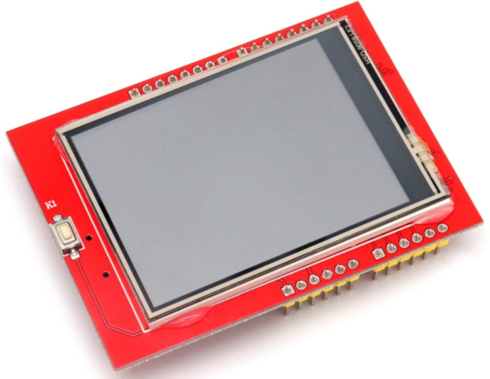
\includegraphics[scale=0.30]{figures/ili9341.png}
        \end{center}
        \caption{Lo schermo ILI9341.}
        \label{fig:ili9341}
    \end{subfigure}
    \hfill
    \begin{subfigure}[b]{0.45\textwidth}
        \begin{center}
            \begin{tikzpicture}[x=0.015cm, y=0.015cm, scale=0.65, transform shape]
                \draw   (120, 90) -- (320,90) -- (320,480) -- (120,480) -- cycle ;

\draw  [fill={rgb, 255:red, 255; green, 255; blue, 255 }  ,fill opacity=1 ]  (90,100)  --  (200,100) -- (200,130) --  (90,130) -- cycle;
\draw  [fill={rgb, 255:red, 255; green, 255; blue, 255 }  ,fill opacity=1 ]  (90,130)  --  (200,130) -- (200,160) --  (90,160) -- cycle;
\draw  [fill={rgb, 255:red, 255; green, 255; blue, 255 }  ,fill opacity=1 ]  (90,160)  --  (200,160) -- (200,190) --  (90,190) -- cycle;
\draw  [fill={rgb, 255:red, 255; green, 255; blue, 255 }  ,fill opacity=1 ]  (90,190)  --  (200,190) -- (200,220) --  (90,220) -- cycle;
\draw  [fill={rgb, 255:red, 255; green, 255; blue, 255 }  ,fill opacity=1 ]  (90,220)  --  (200,220) -- (200,250) --  (90,250) -- cycle;
\draw  [fill={rgb, 255:red, 255; green, 255; blue, 255 }  ,fill opacity=1 ]  (90,250)  --  (200,250) -- (200,280) --  (90,280) -- cycle;
\draw  [fill={rgb, 255:red, 255; green, 255; blue, 255 }  ,fill opacity=1 ]  (90,280)  --  (200,280) -- (200,310) --  (90,310) -- cycle;
\draw  [fill={rgb, 255:red, 255; green, 255; blue, 255 }  ,fill opacity=1 ]  (90,310)  --  (200,310) -- (200,340) --  (90,340) -- cycle;
\draw  [fill={rgb, 255:red, 255; green, 255; blue, 255 }  ,fill opacity=1 ]  (90,340)  --  (200,340) -- (200,370) --  (90,370) -- cycle;
\draw  [fill={rgb, 255:red, 255; green, 255; blue, 255 }  ,fill opacity=1 ]  (90,370)  --  (200,370) -- (200,400) --  (90,400) -- cycle;
\draw  [fill={rgb, 255:red, 255; green, 255; blue, 255 }  ,fill opacity=1 ]  (90,400)  --  (200,400) -- (200,430) --  (90,430) -- cycle;
\draw  [fill={rgb, 255:red, 255; green, 255; blue, 255 }  ,fill opacity=1 ]  (90,430)  --  (200,430) -- (200,460) --  (90,460) -- cycle;

\draw  [fill={rgb, 255:red, 255; green, 255; blue, 255 }  ,fill opacity=1 ] (250,100)  --  (380,100) -- (380,130) --  (250,130) -- cycle;
\draw  [fill={rgb, 255:red, 255; green, 255; blue, 255 }  ,fill opacity=1 ] (250,130)  --  (380,130) -- (380,160) --  (250,160) -- cycle;
\draw  [fill={rgb, 255:red, 255; green, 255; blue, 255 }  ,fill opacity=1 ] (250,160)  --  (380,160) -- (380,190) --  (250,190) -- cycle;
\draw  [fill={rgb, 255:red, 255; green, 255; blue, 255 }  ,fill opacity=1 ] (250,190)  --  (380,190) -- (380,220) --  (250,220) -- cycle;
\draw  [fill={rgb, 255:red, 255; green, 255; blue, 255 }  ,fill opacity=1 ] (250,220)  --  (380,220) -- (380,250) --  (250,250) -- cycle;
\draw  [fill={rgb, 255:red, 255; green, 255; blue, 255 }  ,fill opacity=1 ] (250,250)  --  (380,250) -- (380,280) --  (250,280) -- cycle;
\draw  [fill={rgb, 255:red, 255; green, 255; blue, 255 }  ,fill opacity=1 ] (250,280)  --  (380,280) -- (380,310) --  (250,310) -- cycle;
\draw  [fill={rgb, 255:red, 255; green, 255; blue, 255 }  ,fill opacity=1 ] (250,310)  --  (380,310) -- (380,340) --  (250,340) -- cycle;
\draw  [fill={rgb, 255:red, 255; green, 255; blue, 255 }  ,fill opacity=1 ] (250,340)  --  (380,340) -- (380,370) --  (250,370) -- cycle;


\draw (90,460) node [anchor=north west][inner sep=0.75pt]   [align=left] {$\displaystyle SD\_SCK$};
\draw (90,430) node [anchor=north west][inner sep=0.75pt]   [align=left] {$\displaystyle SD\_DO$};
\draw (90,400) node [anchor=north west][inner sep=0.75pt]   [align=left] {$\displaystyle SD\_DI$};
\draw (90,370) node [anchor=north west][inner sep=0.75pt]   [align=left] {$\displaystyle SD\_SS$};
\draw (90,340) node [anchor=north west][inner sep=0.75pt]   [align=left] {$\displaystyle LCD\_D1$};
\draw (90,310) node [anchor=north west][inner sep=0.75pt]   [align=left] {$\displaystyle LCD\_D0$};
\draw (90,280) node [anchor=north west][inner sep=0.75pt]   [align=left] {$\displaystyle LCD\_D7$};
\draw (90,250) node [anchor=north west][inner sep=0.75pt]   [align=left] {$\displaystyle LCD\_D6$};
\draw (90,220) node [anchor=north west][inner sep=0.75pt]   [align=left] {$\displaystyle LCD\_D4$};
\draw (90,190) node [anchor=north west][inner sep=0.75pt]   [align=left] {$\displaystyle LCD\_D5$};
\draw (90,160) node [anchor=north west][inner sep=0.75pt]   [align=left] {$\displaystyle LCD\_D3$};
\draw (90,130) node [anchor=north west][inner sep=0.75pt]   [align=left] {$\displaystyle LCD\_D2$};

\draw (250,370) node [anchor=north west][inner sep=0.75pt]   [align=left] {$\displaystyle 3.3V$};
\draw (250,340) node [anchor=north west][inner sep=0.75pt]   [align=left] {$\displaystyle 5V$};
\draw (250,310) node [anchor=north west][inner sep=0.75pt]   [align=left] {$\displaystyle GND$};
\draw (250,280) node [anchor=north west][inner sep=0.75pt]   [align=left] {$\displaystyle LCD\_RD$};
\draw (250,250) node [anchor=north west][inner sep=0.75pt]   [align=left] {$\displaystyle LCD\_WR$};
\draw (250,220) node [anchor=north west][inner sep=0.75pt]   [align=left] {$\displaystyle LCD\_RS$};
\draw (250,190) node [anchor=north west][inner sep=0.75pt]   [align=left] {$\displaystyle LCD\_CS$};
\draw (250,160) node [anchor=north west][inner sep=0.75pt]   [align=left] {$\displaystyle LCD\_RST$};
\draw (250,130) node [anchor=north west][inner sep=0.75pt]   [align=left] {$\displaystyle F\_CS$};

            \end{tikzpicture}
        \end{center}
        \caption{Pinout dello schermo \texttt{ILI9341}.}
        \label{fig:pinout_ili}
    \end{subfigure}
\end{figure}

Il terzo componente é un lettore di schede microSD integrato nello schermo
(Fig. \ref{fig:ili9341}). Questo componente é basato sul controller
\texttt{ILI9341} che permette di interfacciarsi con una microSD formattata in
FAT32, sulla quale é possibile salvare file di dimensione massima 4 \texttt{Gb}
e per un totale di 2 \texttt{Tb} di dati.

Per interagire con l'emulatore abbamo utilizzato una tastiera matriciale 4$\times$4
corrispondente alla tastiera esadecimale originale del CHIP-8 (Fig. \ref{fig:4x4_keypad}).

\begin{figure}[h!t]
    \begin{subfigure}[b]{0.45\textwidth}
        \begin{center}
            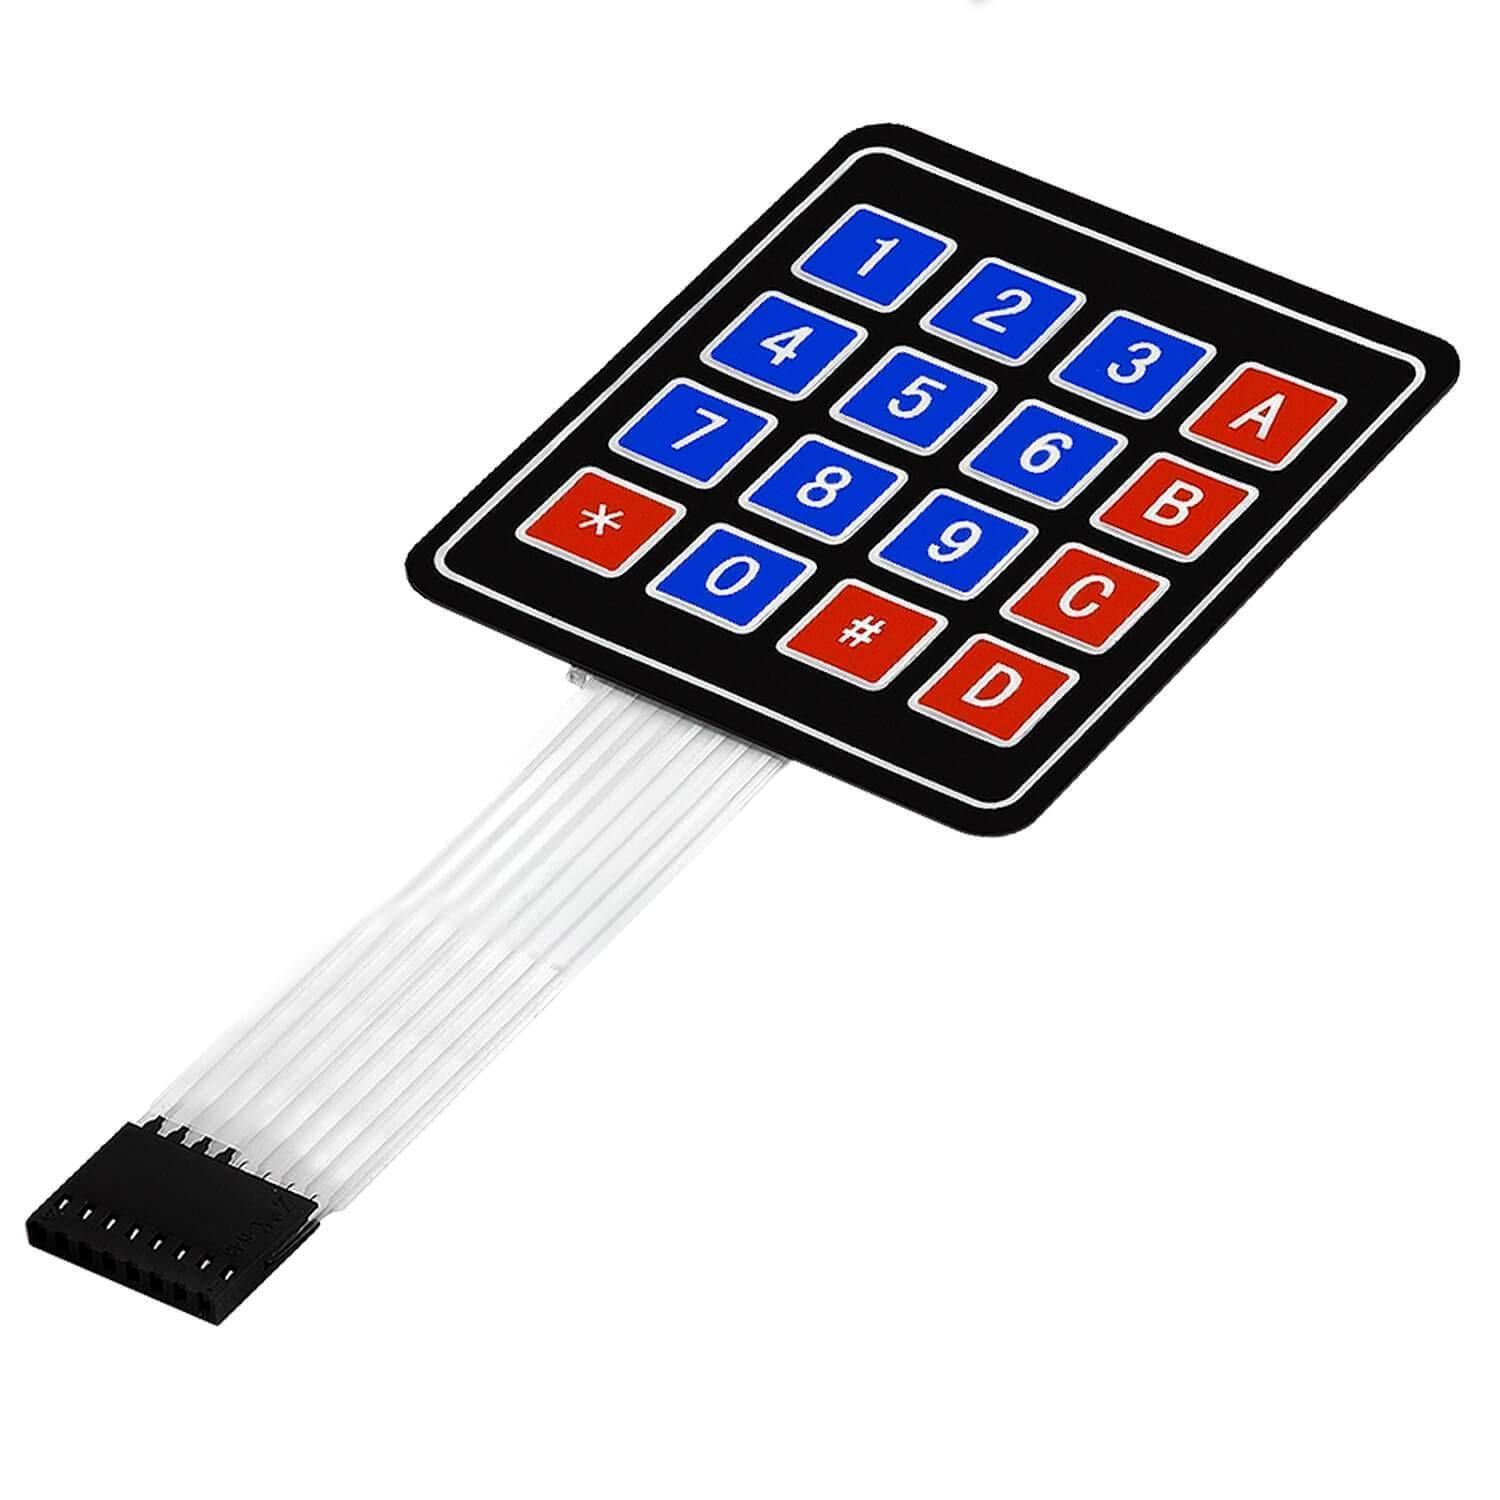
\includegraphics[scale=0.090]{figures/4x4_keypad.jpeg}
        \end{center}
        \caption{Il tastierino matriciale 4$\times$4.}
        \label{fig:4x4_keypad}
    \end{subfigure}
    \hfill
    \begin{subfigure}[b]{0.45\textwidth}
        \begin{center}
            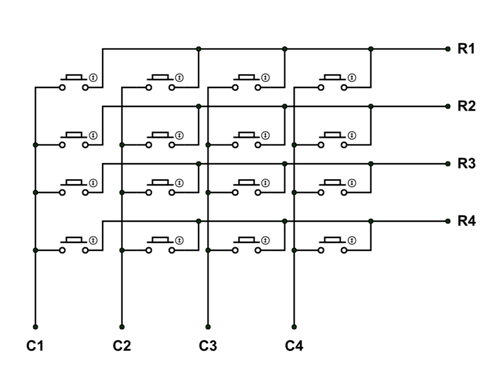
\includegraphics[scale=0.30]{figures/4x4_keypad_structure.png}
        \end{center}
        \caption{Struttura del tastierino matriciale 4$\times$4.}
        \label{fig:4x4_keypad_structure}
    \end{subfigure}
\end{figure}

Come ultimo componenete, per riprodurre gli effetti sonori generati dal gioco
un beeper passivo monotono é stato collegato al microcontrollore tramite un
GPIO output e GND. In CHIP-8 e S-CHIP vi é un solo frequenza che può
essere riprodotta durante tutta l'esecuzione del gioco.

In oltre, abbiamo deciso di aggiungere uno slot per l'alimentazione tramite
due batterie \texttt{AA}.

\subsection{Schema di collegamento}

\textbf{Legenda dei colori in Figura \ref{fig:schematic}}

\begin{itemize}
    \item \textcolor{green}{Verde}: Schermo
    \item \textcolor{blue}{Blu}: Scheda microSD
    \item \textcolor{magenta}{Magenta}: Tastierino
    \item \textcolor{orange}{Arancione}: Beeper
    \item \textcolor{cyan}{Ciano}: Reset
    \item \textcolor{black}{Nero}: GND
    \item \textcolor{red}{Rosso}: Alimentazione
\end{itemize}

\begin{figure}[h!t]
    \begin{center}
        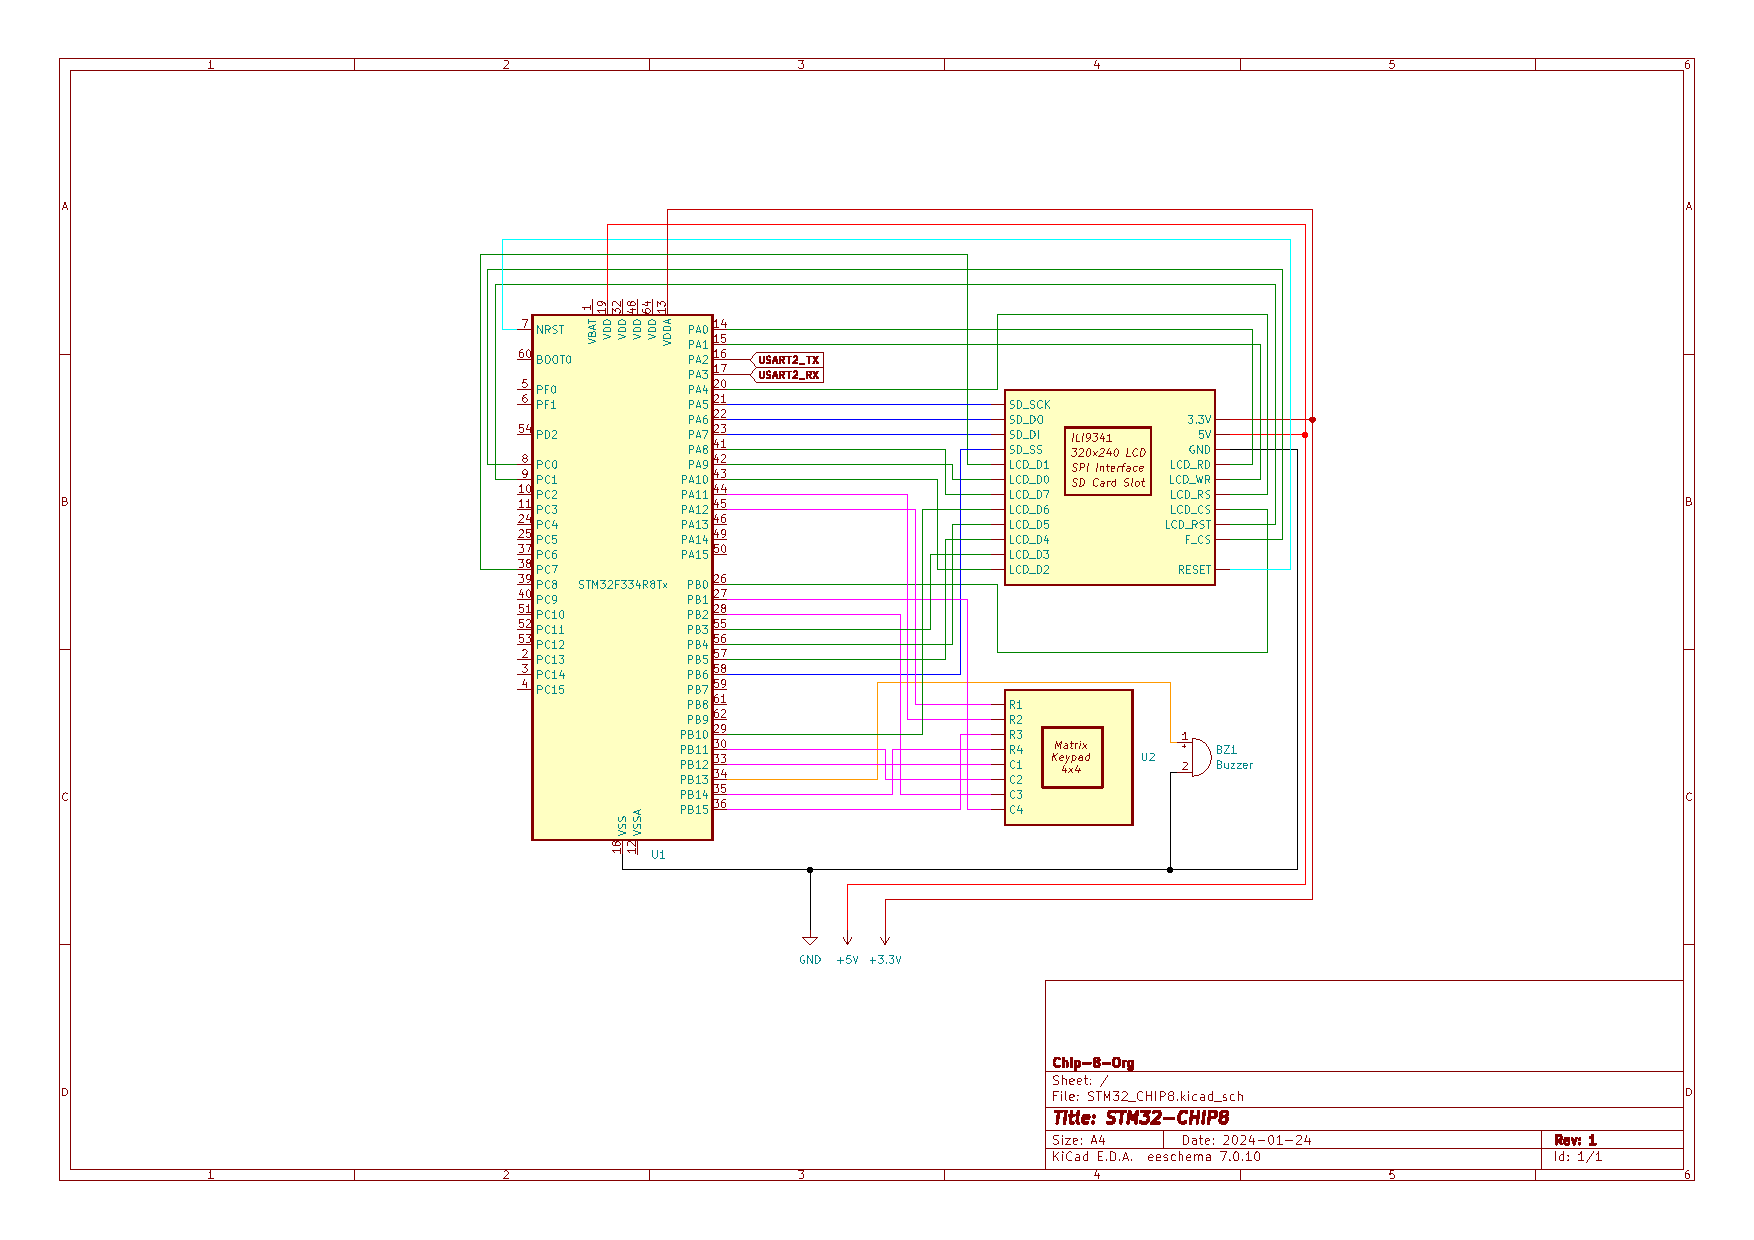
\includegraphics[scale=0.50]{figures/STM32_CHIP8.pdf}
    \end{center}
    \caption{
        Schematic del progetto.
    }
    \label{fig:schematic}
\end{figure}

\subsubsection{Descrizione del collegamento dei componenti}\label{subsubsec:collegamenti}

In Figura \ref{fig:schematic} é possibile vedere lo schema di collegamento
delle componenti utilizzate per la realizzazione del progetto. Per realizzare lo schema é stato utilizzato il software \texttt{KiCad}. E' importante notare, che lo schermo \texttt{ILI9341} e l'integrato lettore di schede microSD, utilizza lo pinout standard degli Shields di Arduino, ovvero un'interfaccia hardware che permette di collegare una scheda Arduino ad un modulo esterno. Quindi, é stato collegato al nostro microcontrollore STM32 utilizzando lo stesso pinout.

Il tastierino matriciale 4$\times$4 é stato collegato al microcontrollore tramite 8 pin GPIO. In particolare i 4 pin relativi alle righe (\texttt{R1}, \texttt{R2}, \texttt{R3}, \texttt{R4}) sono stati impostati in modalitá \texttt{GPIO\_MODE\_IT\_RISING} (interrupt rising edge). Quando si configura un pin GPIO come sorgente di interrupt su un fronte di salita, significa che l'interrupt verrà generato quando il livello logico del pin passa da basso (0) a alto (1). Questo è utile, ad esempio, quando si desidera intercettare un cambiamento di stato su un pulsante quando viene premuto. Invece, i 4 pin relativi alle colonne (\texttt{C1}, \texttt{C2}, \texttt{C3}, \texttt{C4}) sono stati impostati in modalitá \texttt{GPIO\_MODE\_OUTPUT\_PP} (push-pull output) per permettere l'invio dell'interrupt alla pressione di un tasto, dato che chiudendo il circuito permettiamo alla corrente proveniente dal pin GPIO di fluire verso i pin di interrupt. Successivamente, viene identificato il tasto premuto come verra' spiegato nella sezione \ref{subsubsec:keypad}.

L'ultimo componente é il beeper, che é stato collegato al microcontrollore tramite un pin GPIO e GND. Il pin GPIO é stato impostato in modalitá \texttt{GPIO\_MODE\_OUTPUT\_PP} (push-pull output) per permettere l'invio di un segnale al beeper.


\subsection{Componenti utilizzati e relativi costi}

\begin{table}[h!t] % [ht]
    \centering
    \begin{tabular}{|llll|l|}
        \hline
        \multicolumn{1}{|l|}{\textbf{Descrizione}}          & \multicolumn{1}{l|}{\textbf{Modello}}       & \multicolumn{1}{l|}{\textbf{Costo unitario}} & \textbf{Unità} & \textbf{Costo} \\ \hline
        \multicolumn{1}{|l|}{Microcontrollore}       & \multicolumn{1}{l|}{STM32 F334R8T6}         & \multicolumn{1}{l|}{14.99}                   & 1               & 14.99          \\ \hline
        \multicolumn{1}{|l|}{Schermo}                & \multicolumn{1}{l|}{ILI9341 2.4"}           & \multicolumn{1}{l|}{6.50}                    & 1               & 6.50           \\ \hline
        \multicolumn{1}{|l|}{Tastierino}          & \multicolumn{1}{l|}{Matrix keypad 4$\times$4} & \multicolumn{1}{l|}{3.99}                    & 1               & 3.99           \\ \hline
        \multicolumn{1}{|l|}{Beeper}                 & \multicolumn{1}{l|}{}                       & \multicolumn{1}{l|}{0.99}                    & 1               & 0.99           \\ \hline
        \multicolumn{1}{|l|}{Scocca e cablaggio} & \multicolumn{1}{l|}{}                       & \multicolumn{1}{l|}{4.99}                    & 1               & 4.99           \\ \hline
        \multicolumn{4}{|r|}{\textbf{Totale}}                                                      & 31.50\euro    \\ \hline
    \end{tabular}
    \caption{
        Materiali utilizzati per la costruzione del progetto.
    }
    \label{tab:components}
\end{table}

In Tabella \ref{tab:components} é possibile vedere i componenti utilizzati per la realizzazione del progetto. I costi indicati provengono da negozi online come Amazon e eBay.

\section{Software}

Il nostro software si divide in due componenti principali: l'interprete CHIP-8 e l'infrastruttura necessaria per "portarlo" sul microcontrollore STM32, ovvero l'interfaccia con lo schermo e i gestori per la scheda microSD, per il keypad e per il beeper come gia' anticipato nella sezione \ref{sec:hardware}.

\subsection{Interprete/Emulatore CHIP-8}

Un emulatore è un software progettato per replicare il funzionamento di un processore e di altre componenti di un sistema informatico, consentendo così l'esecuzione di programmi scritti per un'architettura specifica su un'altra architettura. Lo sviluppo di un emulatore richiede una dettagliata comprensione dell'architettura da emulare, il che è al di là dello scopo di questo corso.

Nonostante questo, abbiamo deciso di scrivere l'interprete da zero e per farlo è stato necessario consultare le specifiche (de facto standard) che definiscono il comportamento di un interprete CHIP-8 \cite{cowgod:chip8} e S-CHIP \cite{cowgod:schip}.

L'interprete ha un'architettura basata su registri e possiede 4 KB di memoria, 16 registri general purpose, un registro per gli indirizzi di memoria, un registro per il delay timer, un registro per il sound timer, uno stack per gestire le chiamate a subroutine, uno stack pointer e un program counter, come si puo` vedere nel listato \ref{chip8_struct}.

\begin{Listing}[h!t] % [ht]
    \centering
    \showc*[.8\textwidth]{chip8_struct.c}
    \caption{Struttura dell'emulatore Chip8}
    \label{chip8_struct}
\end{Listing}

Il delay timer viene utilizzato come cronometro mentre il sound
timer è utilizzato per gestire gli effetti sonori, quando il suo
valore è diverso da zero, l'emulatore attiva il beeper.

Ad ogni ciclo di esecuzione l'interprete effettua il fetch
dell'istruzione puntata dal program counter in memoria,
la decodifica e la esegue.

Sono supportate 45 istruzioni diverse, ciascuna delle
quali è rappresentata da uno specifico opcode in cui al suo interno
sono passati anche eventuali parametri.

Il programma è scritto in C99, non ha I/O ed è freestanding
\cite{n1256:conformance}, ovvero non dipende dalla libreria
standard del C (libc). Tutto questo è mirato a rendere l'interprete
altamente portabile.

Per rimuovere la dipendenza da libc è stato necessario includere alcune funzioni direttamente da libgcc, in particolare abbiamo re-implementato le funzioni \texttt{memset} e \texttt{memcpy} . Inoltre, abbiamo trovato un modo alternativo per implementare le asserzioni e includere una funzione ad hoc per la generazione di numeri pseudo-casuali come si puo' vedere nel listato \ref{assert_rand}.

TODO SPIEGARE IL CODICE

\begin{Listing}[h!t]
\centering
\mbox{
  \showc[.45\textwidth]{assert.c}
  \quad
  \showc[.50\textwidth]{random.c}
}
\caption{Implementazioni di \texttt{ASSERT} e \texttt{rand\_byte}.}
\label{assert_rand}
\end{Listing}

Infine per testare più comodamente l'interprete abbiamo sviluppato un semplice emulatore su desktop utilizzando SDL2 \cite{libsdl:about}, una libreria scritta in C che consente di gestire audio, video e input da tastiera. In seguito l'interprete è stato sottoposto ad un'apposita test suite \cite{github:chip8-test-suite} che mira a verificare il comportamento corretto di ciascun opcode.

\subsubsection{Gestione del timing}

Uno dei problemi principali durante lo sviluppo di un emulatore è la gestione del timing, in particolare è necessario limitare la "velocità" dell'emulatore bloccando temporaneamente la sua esecuzione.

Inoltre abbiamo dovuto disaccoppiare la frequenza dell'interprete (regolabile dal giocatore) dalla frequenza del delay timer e del sound timer (costante a 60 Hz). Dove con frequenza dell'interprete ci riferiamo al numero di istruzioni che esegue ogni frame.

% Durante lo sviluppo abbiamo testato due soluzioni diverse.

Inizialmente abbiamo optato per la gestione di una singola istruzione per ciclo di esecuzione, di conseguenza il ritardo del game loop risultava variabile e dipendeva dalla frequenza selezionata dal giocatore. Per assicurare una frequenza $\mathcal{F}$ di 60 Hz i timer venivano decrementati ogni n-esima iterazione del game loop, dove $n = \frac{\mathcal{F}}{60}$. Ad esempio se $\mathcal{F} = 540$, i timer venivano decrementati ogni $9^{\circ}$ ciclo.

Purtroppo però questo approccio presenta un problema non trascurabile, ovvero effettua una chiamata ad una funzione simil-sleep per un periodo molto breve dopo ogni istruzione. Ad esempio se $\mathcal{F} = 540$, il ritardo di una sleep sarebbe solo di 1.85 ms, e questo genere di funzione non offre una precisione simile. Per questo motivo abbiamo optato per una soluzione differente.

Abbiamo fissato il ritardo del game loop a 16.666 ms, un valore sufficientemente alto da non avere problemi di granularità. Inoltre in questo modo otteniamo un frame rate di 60 fps esatti. Avendo reso il ritardo costante abbiamo dovuto rendere variabile il numero di istruzioni gestite durante un ciclo di esecuzione. In particolare vengono gestite n istruzioni per ciclo, dove $n = \frac{\mathcal{F}}{60}$. Ad esempio se $\mathcal{F} = 540$, vengono gestite 9 istruzioni per ciclo. A questo punto dato che il game loop viene ripetuto con una frequenza di 60 Hz risulta banale gestire la frequenza dei timer.

Sono state considerate anche eventuali problematiche che sarebbero potute sorgere con questo approccio. In particolare non tutte le istruzioni impiegano lo stesso tempo per essere eseguite, ma fortunatamente anche l'istruzione più lenta richiede una quantità trascurabile di tempo. Ciò significa che possiamo comportarci come se tutte le istruzioni richiedessero il medesimo tempo.

\subsubsection{Ottimizzazioni}


È stato necessario introdurre delle ottimizzazioni all'interno dell'interprete per poterlo far girare su un microcontrollore.

L'ottimizzazione principale è legata alla rappresentazione dello schermo in memoria. Ad alto livello lo schermo può essere visto come una matrice di 128x64 pixel monocromi. Una rappresentazione simile occuperebbe 8192 byte, dato che ciascun pixel verrebbe rappresentato da un byte.

\begin{figure}[h!t]
    \begin{center}
        % 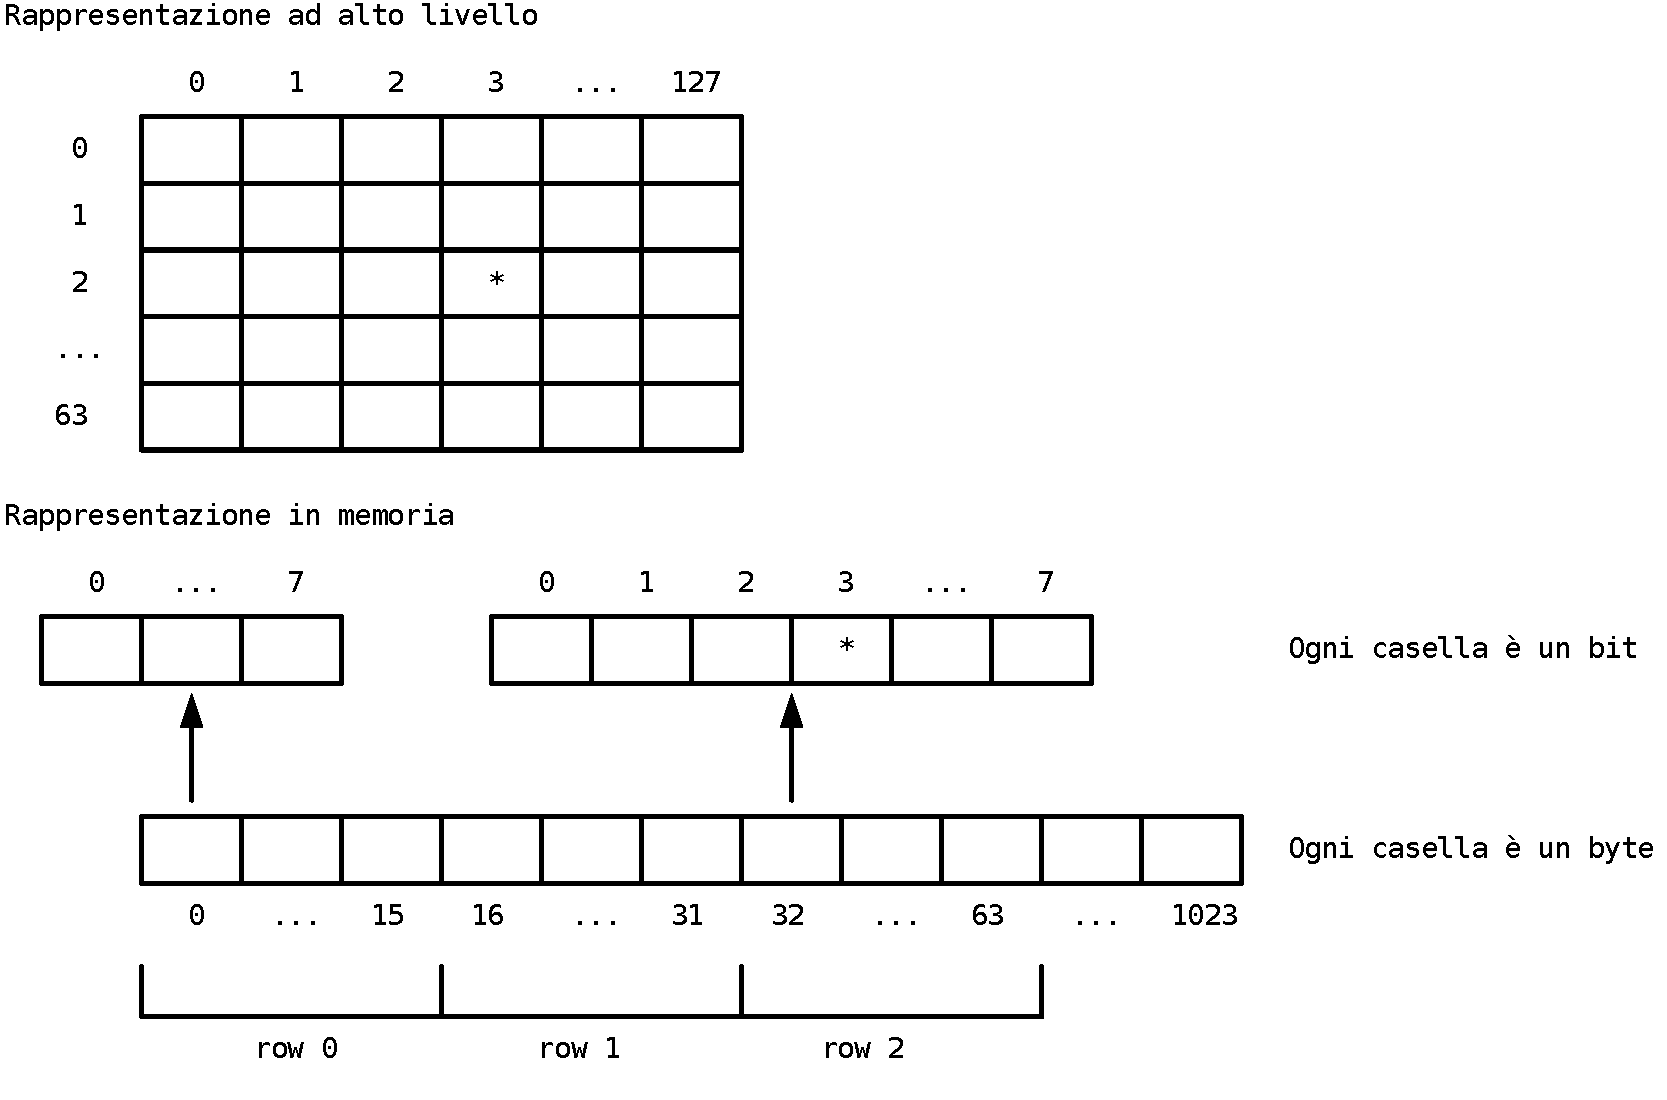
\includegraphics[scale=0.3]{figures/screenopt.pdf}
        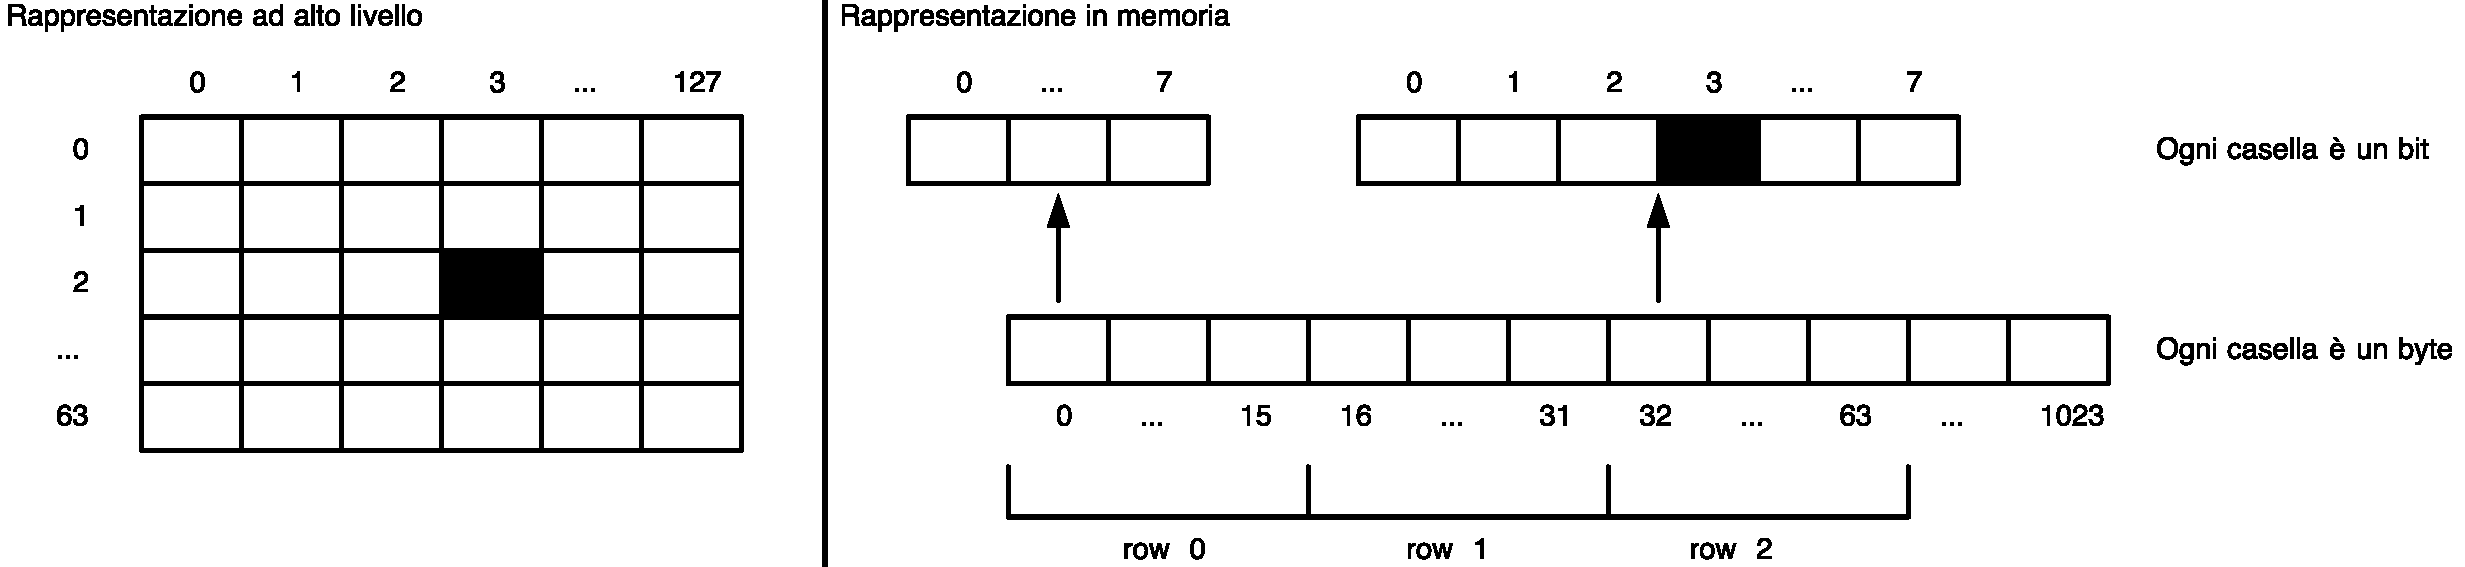
\includegraphics[scale=0.38]{figures/screenopt_small.pdf}
    \end{center}
    \caption{Esempio della mappatura di un pixel.}
    \label{fig:screenopt}
\end{figure}

Purtroppo il nostro microcontrollore ha a disposizione solamente 16 KB di SRAM, di conseguenza una soluzione simile non è praticabile.

Per questo motivo abbiamo deciso di rappresentare lo schermo come un array unidimensionale di 1024 byte, dove ciascun pixel viene rappresentato da un singolo bit. In questo modo otteniamo un risparmio di spazio pari a ben l'87.5\%.

Questa decisione ha aggiunto però un livello di indirezione dato che una coordinata ad alto livello sulla matrice 128x64 é mappata ad una coordinata "in memoria", dove la prima componente é l'indice del byte nell'array unidimensionale e la seconda componenete é il bit all'interno del byte. La figura [\ref{fig:screenopt}] mostra un esempio di mappatura di un pixel. Piú precisamente la funzione $F$ é definita come segue:
\begin{gather*}
    F: \mathbb{N} \times \mathbb{N} \rightarrow \mathbb{N} \times \mathbb{N} \\
    F(x, y) = \left(\left\lfloor \frac{128y + x}{8} \right\rfloor, 7 - (x \bmod 8)\right) \\
    where \quad x \in [0, 127] \quad y \in [0, 63]
\end{gather*}

Un'ulteriore ottimizzazione viene resa disponibile attraverso l'API dell'interprete sotto forma di una funzione che consente al chiamante di controllare se l'array che rappresenta lo schermo è stato modificato nell'ultimo ciclo di esecuzione. Avendo notato che il numero di opcode che modificano lo schermo è molto limitato, precisamente sono solo 7 su 45, questa funzione consente di ridurre di 6.42 volte il numero di volte in cui
lo schermo viene aggiornato.


\subsubsection{Comportamenti ambigui}

Gli interpreti CHIP-8 e S-CHIP hanno sviluppato molteplici comportamenti ambigui nel corso degli anni. Questi cosiddetti ``quirk'' variano in base alle piattaforme per cui è stato sviluppato l'interprete. Ad esempio gli interpreti per calcolatrici HP48 presentano un comportamento leggermente diverso durante l'esecuzione delle istruzioni di SHIFT.

Questi comportamenti ambigui si propagano fino ai programmatori
CHIP-8 che si appoggiano a quest'ultimi e scrivono videogiochi che
non sono del tutto compatibili con interpreti più vecchi. Per evitare
questa frammentazione è necessario supportare le piattaforme
principali e i loro quirk.

Il nostro interprete supporta CHIP-8, CHIP-48, S-CHIP 1.0 e
S-CHIP 1.1, in questo modo è in grado di eseguire la stragrande
maggioranza dei videogiochi reperibili in rete.

\subsection{Porting su STM32}

Dopo aver sviluppato l'emulatore, abbiamo sviluppato un'infrastruttura per poterlo eseguire sul microcontrollore STM32.
Come già anticipato nella sezione \ref{sec:hardware}, l'infrastruttura si compone di un'interfaccia con lo schermo, un gestore per la scheda microSD, un gestore per il tastierino e un gestore per il beeper.

E' utile ricordare che l'emulatore che abbiamo sviluppato é stato progettato per essere eseguito su qualunque architettura hardware in per cui é compilabile un file C, quindi non é stato necessario apportare modifiche all'interprete per poterlo eseguire sul microcontrollore STM32.

Quindi, il processo di adattamento di questo emulatore per il microcontrollore è stato relativamente semplice e non ha richiesto modifiche significative. Tuttavia, in quanto l'emulazione avvieve su una architettura con potenza di calcolo limitata rispetto a quella di un comune calcolatore, le prestazioni e la fluiditá dell'emulatore sono inferiori rispetto a quelle che avevamo usando SDL2.


\subsubsection{Architettura software}

In Figura \ref{fig:class_diagram} é possibile vedere il ``class'' diagram riferito al porting dell'emulatore su STM32. L'architettura é composta da 5 componenti principali: \texttt{Chip8}, \texttt{Screen}, \texttt{SD}, \texttt{Keypad} e \texttt{Beeper} poi utilizzati in figura \ref{fig:sequence_diagram} per mostrare come questi interagiscono tra di loro.

Il \texttt{menu}, a differenza dello studio di fattibilita', e' stato rimosso dalle figure dato che tutte le operazioni che lo coinvolgono sono state spostate all'interno del \texttt{main}.

\begin{figure}[h!t]
    \begin{center}
        \begin{tikzpicture}[scale=0.6, transform shape]
            \renewcommand{\umltextcolor}{black}
\renewcommand{\umldrawcolor}{black}
\renewcommand{\umlfillcolor}{white}

  \begin{class}[text width=2cm]{Main}{6,0}
    \operation{+ main()}
  \end{class}

  \begin{class}[text width=3cm]{Keypad}{0,-2}
      \operation{+ interrupt()}
      \operation{+ \sout{polling()}}
  \end{class}

  \begin{class}[text width=1.7cm]{Chip8}{3,-3}
    \operation{+ init()}
    \operation{+ cylce()}
    \operation{+ ended()}
  \end{class}


  \begin{class}[text width=3.5cm]{ILI9341}{6, -4}
    \operation{+ init(\texttt{Pin[13]})}
    \operation{+ drawMenu(\texttt{char*[]})}
    \operation{+ fillScreen(\texttt{uint16\_t})}
    \operation{+ drawGame(\texttt{char[]})}
  \end{class}

  \begin{class}[text width=1.7cm]{Beeper}{9,-3}
      \operation{+ high()}
      \operation{+ low()}
  \end{class}

  \begin{class}[text width=3cm]{SD}{12, -2}
    \operation{+ mount()}
    \operation{+ open()}
    \operation{+ read()}
    \operation{+ readFile(\texttt{char[]})}
    \operation{+ close()}
  \end{class}

  % \begin{class}[text width=2.4cm]{Menu}{10,0}
  %     \operation{+ loadGame()}
  % \end{class}

    % \draw [umlcd style dashed line , ->] (Menu) -- node [ above , sloped , black ]{} (Keypad) ;
    % \draw [umlcd style dashed line , ->] (Menu) -- node [ above , sloped , black ]{} (SD) ;
    % \draw [umlcd style dashed line , fill=white, ->] (Menu) -- node [ below  , black ]{} (ILI9341) ;

    % \draw [umlcd style dashed line , ->] (Main) -- node [ above , sloped , black ]{} (Menu) ;
    \draw [umlcd style dashed line , ->] (Main) -- node [ above , sloped , black ]{} (Chip8) ;
    \draw [umlcd style dashed line , ->] (Main) -- node [ above , sloped , black ]{} (Keypad) ;
    \draw [umlcd style dashed line , ->] (Main) -- node [ above , sloped , black ]{} (Beeper) ;
    \draw [umlcd style dashed line , fill=white, ->] (Main) -- node [ below , sloped , black ]{} (SD) ;
    \draw [umlcd style dashed line , fill=white, ->] (Main) -- node [ below , sloped , black ]{} (ILI9341) ;

    \begin{scope}[xshift=0cm, yshift=0cm] % Adjust the positioning of the legend
    % Legend title
    \node[font=\bfseries] at (0, 0) {Legend};
    % Legend items
    \draw [umlcd style dashed line , fill=white, ->] (0, -0.5) -- (1, -0.5) node[right,  black] {Uses};
    \end{scope}

  % \draw [ umlcd style , ->] (Main) -- node [ above , sloped , black ]{$ < <$ import $ > >$} (Student) ;

        \end{tikzpicture}
    \end{center}
    \caption{
        Class diagram dell'architettura software.
    }
    \label{fig:class_diagram}
\end{figure}

Il flusso di esecuzione dell'emulatore é mostrato in Figura \ref{fig:sequence_diagram}, come si puo' notare e' diviso in due parti. In particolare, la prima inizia con la lettura dei file presenti sulla scheda microSD, successivamente il giocatore seleziona il gioco da eseguire e altre informazioni come la velocitá di esecuzione e la modalitá di esecuzione. Successivamente, l'emulatore inizia l'esecuzione del gioco selezionato. Mentra la seconda parte mostra il flusso di esecuzione dell'emulatore durante l'esecuzione del gioco.

\begin{figure}[h!t]
    \begin{center}
        \resizebox{0.6\textwidth}{!}{%
        \begin{sequencediagram}
        \newthread{main}{:Main}
        % \newinst[0.5]{menu}{:Menu}
        \newinst[0.5]{vm}{:Chip8}
        \newinst[0.5]{lcd}{:ILI9341}
        \newinst[0.5]{kp}{:Keypad}
        \newinst[0.5]{beep}{:Beeper}
        \newinst[0.5]{sd}{:SD}

        \begin{call}{main}{mount(); open(); read();}{sd}{}
        \end{call}
        \begin{sdblock}{Game Selection Loop (Menu)}{}
            \begin{call}{main}{interrupt()}{kp}{}
            \end{call}
            \begin{call}{main}{drawMenu(\texttt{char*[]})}{lcd}{}
            \end{call}
        \end{sdblock}
        \begin{call}{main}{readFile(\texttt{char[]})}{sd}{}
        \end{call}

        \begin{call}{main}{init()}{vm}{}
        \end{call}

        \begin{sdblock}{Main Loop}{}
            \begin{call}{main}{interrupt()}{kp}{}
            \end{call}
            \begin{call}{main}{cycle()}{vm}{}
            \end{call}
            \begin{call}{main}{high() / low()}{beep}{}
            \end{call}
            \begin{call}{main}{drawGame(\texttt{char[]})}{lcd}{}
            \end{call}
        \end{sdblock}
        \end{sequencediagram}
    }

    \end{center}
    \caption{
        Sequence diagram dell'architettura software.
    }
    \label{fig:sequence_diagram}
\end{figure}

\subsubsection{Interfaccia con la scheda microSD}\label{subsubsec:sd}

Inizialmente, la scheda é stata formattata in FAT32 e sono stati caricati i file dei giochi. Successivamente, la scheda é stata inserita nello slot della scheda microSD integrato nello schermo.

\begin{Listing}[h!t] % [ht]
    \centering
    \setminted[c]{escapeinside=@@}
    \showc*[.55\textwidth]{load_game.c}
    \caption{Caricamento di un gioco dalla scheda microSD.}
    \label{load_game}
\end{Listing}

La scheda microSD é stata gestita tramite la libreria \texttt{FatFs} \cite{elm-chan:fatfs}, una libreria open source che consente di interfacciarsi con filesystem FAT12, FAT16 e FAT32. Questa libreria é stata sviluppata da ChaN, un \textit{mediocre\footnote{\url{http://elm-chan.org/profile_e.html}} embedded system engineer} giapponese che ha sviluppato anche la libreria \texttt{Petit FatFs} per microcontrollore con risorse limitate.
Per la comunicazione tra il microcontrollore e la scheda microSD é stato utilizzato il protocollo \textit{Serial Periferal Interface} (SPI), in particolare il microcontrollore é stato configurato come master e la scheda microSD come slave. L'interfaccia SPI é nota per non utilizzare indirizzi ma rimane un protocollo valido per la comunicazione su bus.

A livello software abbiamo letto tutti i file presenti sulla scheda microSD e li abbiamo memorizzati in un vettore. Questo per avere la possibilitá di selezione e successivamente l'aperura del file selezionato.

Nel listato \ref{load_game} é possibile vedere il codice che consente di caricare un gioco dalla scheda microSD. E' importante notare che a riga 12 il file viene spostato nella virtual machine, precisamente viene settato il campo \texttt{RAM} della struct \texttt{Chip8} parendo da \texttt{PC\_OFFSET} che di default é settato a \texttt{0x200} come mostrato nel listato \ref{chip8_struct}. Successivamente, deallocando lo spazio utilizzato temporaneamente per memorizzare il file riusciamo a manterenere il livello di memoria utilizzata pari a quella della struttura dell'emulatore, vale a dire costante.

\textbf{Ottimizzazione} \quad  Una piccola ottimizzazione, ma non da sottovalutare, é stata quella di non abilitare il Long File Names (LFN) sul filesystem FAT32 della scheda microSD. Questo implica il fatto che tutti i file devono avere un nome di al massimo 13 byte (caratteri ASCII). Cosi' facendo abbiamo risparmiato in termini complessitá di computazione, memoria flash e SRAM.

\subsubsection{Menu di selezione}

La selezione del gioco avviene tramite un menù di selezione. Il menu e' composto da una lista di giochi presenti sulla scheda microSD suddivisi in varie pagine e da una sezione per la selezione selezione per la velocitá di esecuzione e la modalitá di esecuzione.

Si puo' notare nel listato \ref{menu} che la selezione del gioco avviene tramite il tastierino, in particolare i tasti \texttt{7} e \texttt{15} permettono di navigare tra le pagine. Il tasto \texttt{0} permette di selezionare la modalitá di esecuzione ciclando tra le 3 modalitá disponibili: \texttt{CHIP8}, \texttt{SCHIP1.0} e \texttt{SCHIP1.1}; invece, il tasto \texttt{8} permette di selezionare la velocitá di esecuzione ciclando tra le 4 preimpostate \texttt{600}, \texttt{1200}, \texttt{1800} e \texttt{2400}. Gli altri tasti sono riservati per avviare il gioco selezionato.

\begin{Listing}[h!t] % [ht]
    \centering
    \setminted[c]{escapeinside=@@}
    \showc*[.92\textwidth] {menu.c}
    \caption{Menu di selezione.}
    \label{menu}
\end{Listing}

Per ovviare al fatto che cambiando schermata potrebbero rimanere degli artefatti grafici, abbiamo deciso di pulire lo schermo ad ogni cambio di schermata. Questo é stato possibile grazie alla funzione \texttt{FillScreen}, la quale utilzza metodi dell'\textit{Hardware Abstract Layer} (HAL) per pulire lo schermo producendo anche un effetto di transizione tra una scheda e l'altra.

\subsubsection{Funzionamento del keypad}\label{subsubsec:keypad}

Inizialmente il keypad é stato gestito tramite polling, ovvero il microcontrollore controllava ad ogni aggiornamento dello schermo (60 \texttt{FPS} $\approx$ 16.666 ms) lo stato dei pin di riga e di colonna per capire quale tasto fosse stato premuto. Questo approccio é stato scartato in favore dell'approccio basato su interrupt, in quanto il polling consumava molte risorse del microcontrollore e non garantiva un framerate stabile in quanto in $\sim$16 ms non riusciva a garantire la lettura di tutti i pin ed eseguire le restanti operazioni.

La procedura di gestione degli interrupt su microcontrollori STM32 é standard. Bisogna implementare una funzione che gestisce l'interrupt e bisogna configurare il pin GPIO come sorgente di interrupt. Nel nostra situzione, come accennato in sezione \ref{subsubsec:collegamenti}, i pin di riga sono stati impostati in modalitá \texttt{GPIO\_MODE\_IT\_RISING} (interrupt rising edge) e i pin di colonna in modalitá \texttt{GPIO\_MODE\_OUTPUT\_PP} (push-pull output) per permettere l'invio dell'interrupt alla pressione di un tasto.

Successivamente, viene capito quale tasto é stato premuto, leggendo il valore dei pin di riga e di colonna. Per fare ció, i pin di riga sono stati impostati in modalitá \texttt{GPIO\_MODE\_INPUT}. Come si puo' vedere nel listato \ref{keypad} a riga 1, nella routine di interrupt viene abilitato il pin di output della prima colonna e in seguito per ogni riga viene letto il valore del pin di input per conoscere la seconda coordinata del tasto premuto, e in caso sia premuto viene salvato nella struttura dati apposita nella virtual machine. Questa operazione viene ripetuta per ognuna delle quattro colonne.
Al termine della routine di interrupt (\inlinec{void Interrupt_handle_keypad(uint16_t GPIO_Pin)}), i pin di riga vengono re-impostati in modalitá \texttt{GPIO\_MODE\_IT\_RISING} per permettere l'invio dell'interrupt alla pressione di un nuovo tasto.

\begin{Listing}[h!t] % [ht]
    \centering
    \setminted[c]{escapeinside=@@}
    \showc*[.87\textwidth]{keypad.c}
    \caption{Gestione dell'interrupt del keypad.}
    \label{keypad}
\end{Listing}

\subsubsection{Interfaccia con lo schermo}

Il driver per display a cristalli liquidi \texttt{ILI9341} consente la comunicazione tramite due diverse interfacce: SPI (spiegata in sezione \ref{subsubsec:sd}) e 8 bit parallela. Mentre l'interfaccia SPI richiede meno pin, è più lenta a causa del protocollo seriale. Al contrario, l'interfaccia parallela è più veloce ma richiede più pin. Poiché dobbiamo visualizzare i videogiochi sullo schermo e aggiornare l'immagine a circa 60 volte al secondo, abbiamo optato per l'interfaccia parallela.

L'interfaccia parallela è un metodo di comunicazione che coinvolge l'invio simultaneo di più bit di dati attraverso una serie di linee di comunicazione parallele. Nel contesto del display LCD ILI9341, l'interfaccia parallela ad 8 bit coinvolge l'uso di otto linee di dati per trasmettere informazioni al display. Oltre alle linee di dati, ci possono essere anche altre linee di controllo, come quelle per il segnale di sincronizzazione e i segnali di controllo. Quando si utilizza l'interfaccia parallela, i dati vengono inviati al display in gruppi di 8 bit simultaneamente, consentendo un trasferimento più rapido rispetto all'interfaccia SPI, che invia i dati bit per bit in sequenza.

Per l'nizializzazione abbiamo utilizzato la funzione \inlinec{int Init(struct ILI9341_t *ili, struct ILI9341_Pin_t {D7, D6, D5, D4, D3, D2, D1, D0, RST, CS, RS, WR, RD})}, prende in input un puntatore alla struttura dati relativa alla scheda e i pin utilizzati per la comunicazione parallela. Gli ultimi cinque pin elencati nella firma della funzione sono stati inizializzati in modalitá \texttt{GPIO\_MODE\_OUTPUT\_PP} grazie alle funzioni della HAL.

Quindi, prima di inviare la sequenza di inizializzazione al display, è necessario impostare uno stato iniziale per la scheda. Questo stato prevede che il pin \texttt{LCD\_CS} sia impostato su LOW, mentre i pin \texttt{LCD\_WR} e \texttt{LCD\_RD} devono essere disabilitati. Il pin \texttt{LCD\_RST} è utilizzato per resettare lo stato interno del display quando è attivo, conosciuto anche come \textit{hardware reset}. Per garantire un avvio sicuro, attiviamo e disattiviamo questo pin per resettare la scheda a uno stato noto. Successivamente, il pin \texttt{LCD\_RST} rimarrà disabilitato per tutta l'esecuzione.

Una fase molto importante e' riservata all'invio della \textit{init sequence}.
Di base lo schermo e' in modalitá \textit{sleep}, quindi dobbiamo mandare una sequenza di comandi per risvegliarlo. Questa sequenza di comandi é specifica per il display \texttt{ILI9341} ed sono spiegati dettagliatamente nel datasheet \cite{ili9341}. Questi comandi sono stati inviati al display tramite la funzione \inlinec{void WriteCommand(struct ILI9341_t *ili, uint8_t cmd)}. Oltre al comando di \textit{wake up}, e' stato eseguito il \texit{reset software}, l'impostazione del \textit{power control} e la quantita' di bit per il colore del pixel (16 bit). Tralasciando qualche comando, in fine abbiamo iniviato il comando di \textit{display on}.

\begin{Listing}[h!t] % [ht]
    \centering
    \setminted[c]{escapeinside=@@}
    \showc*[.65\textwidth] {ili9341_printscreen.c}
    \caption{Funzione per la stampa dello schermo.}
    \label{ili9341_printscreen}
\end{Listing}

Nel file relativo allo schermo, abbiamo implementato diverse funzioni per gestirlo. In particolare, la funzione nel listato \ref{ili9341_printscreen} e' stata la prima implementazione capace di stampare lo schermo. Successivamente, abbiamo basato le altre implementazioni su quest'ultima aggiungendo delle \textit{features}.
Gli elementi comuni a tutte le funzioni di stampa sono la chiamata della funzione \inlinec{SetDrawingArea} che definisce i vertici del rettangolo da disegnare e la chiamata della funzione \inlinec{WriteCommand} con argomento \inlinec{CMD_MEMORY_WRITE} per indicare al display che stiamo per inviare dei dati.

Tra le necessita' che avevamo dopo questa implementazione, c'era quella di poter stampare un'immagine piu' grande. In questi termini abbiamo implementato una versione migliorata, la quale accetta in input anche un parametro di \textit{scale}.

% Parlare di bare metal
% mettere codice dei due pin write metal
% Parlare del font



% TODO: aggiornare il class diagram e il sequence diagram

% \section{Assemblaggio}

% TODO release

\section{Analisi del consumo energetico} % ALT: Alimentazione e consumi

% TODO

\section{Considerazioni finali} % ALT: Conclusioni e sviluppi futuri

\section{Sviluppi futuri}

Aggiornare solo la sprite che è stata modificata.

% TODO

\addcontentsline{toc}{section}{Riferimenti bibliografici}
\bibliographystyle{plain}
\bibliography{report}

\end{document}
